\section{Design Requirements}

This refined the previous, investigative research question into:
\begin{center}
    \textbf{How might an integrated image-detection dataset construction engine, combined with deep-learning evaluation and workflow prototyping, overcome the structural barriers to detecting and operationalizing disposable vapes as hazardous micro-e-waste in UAV-oriented imagery for UK urban environments?}
\end{center}

The research question was broken into three sub-research questions (SRQ) to distinguish the three-streamed approach of the paper.

\textbf{SRQ 1: The Dataset Construction Engine (DCE)} 
How might we create an integrated dataset construction engine to bypass manual bottlenecks and improve the sourcing, annotation, metadata richness, and model-readiness of fragmented micro-WEEE imagery?
\begin{table}[H]
\centering
\scriptsize
\renewcommand{\arraystretch}{1.4}
\begin{tabularx}{\textwidth}{@{} p{0.10\textwidth} p{0.18\textwidth} X p{0.28\textwidth} @{}}
\toprule
\textbf{ID} & \textbf{Core Feature} & \textbf{Success Criterion} & \textbf{Validation Method} \\
\midrule
\textbf{DCE-DR1} & \textbf{Multi-Source Sourcing} & System aggregates uploads, video frames, and web scrapes efficiently, successfully intercepting duplicates before they reach the staging pool. & Quantitative evaluation of ingestion efficiency via calculated Upload Speed ($U_s$) and duplicate interception rates. \\
\addlinespace
\textbf{DCE-DR2} & \textbf{Synthetic Generation} & The bounded 2D cutout controls must produce viable, realistic training candidates rather than unusable algorithmic artifacts. & Quantitative evaluation via the Synthetic Acceptance Rate ($A_s$), proving a high yield of user-promoted composites. \\
\addlinespace
\textbf{DCE-DR3} & \textbf{Curation \& Dataset Balance} & The Review Queue must resolve the staging bottleneck, allowing rapid classification (Pos/Neg/Reject) to actively balance the dataset. & Evaluation of Curation Throughput ($C_t$) to prove the hotkey UI significantly accelerates processing compared to standard drag-and-click sorting. \\
\addlinespace
\textbf{DCE-DR4} & \textbf{SAM2 Annotation} & SAM2 integration must mathematically reduce the mechanical fatigue and time penalty associated with manual polygon tracing. & Interaction metrics proving high First-Click Accuracy ($FCA$) and substantial Time Reduction ($TR$) vs. manual baselines. \\
\addlinespace
\textbf{DCE-DR5} & \textbf{Metadata Tagging} & VLM integration must successfully automate contextual failure-mode tagging without exhausting the user with API failures. & Quantitative evaluation of VLM API reliability and resulting dataset Metadata Coverage ($M_c$) across defined environmental fields. \\
\addlinespace
\textbf{DCE-DR6} & \textbf{YOLO Export Integrity} & The system must seamlessly translate the COCO source of truth into edge-ready YOLO configurations without data loss. & End-to-end dataset integrity evaluation demonstrating a 0\% error/skip rate during deep-learning model ingestion. \\
\bottomrule
\end{tabularx}
\caption{Feature-centric Design Requirements for the Dataset Construction Engine (DCE).}
\label{tab:dr_dce}
\end{table}


\textbf{SRQ 2: Machine Perception and Edge Evaluation} 
How might we train a lightweight edge-vision architecture on a dedicated vape litter dataset to improve the detection-readiness of disposable vapes in urban environments?
\begin{table}[H]
\centering
\scriptsize
\renewcommand{\arraystretch}{1.4}
\begin{tabularx}{\textwidth}{p{0.08\textwidth} p{0.18\textwidth} X p{0.26\textwidth}}
\toprule
\textbf{ID} & \textbf{Experimental Goal} & \textbf{Success Criterion} & \textbf{Validation Method} \\
\midrule
\textbf{EVAL-DR1} & \textbf{Dataset Scale \& Assembly} & Construct a leakage-aware, two-class dataset whose total instance volume (e.g., >1,000 target boxes) is competitive with existing UAV micro-litter literature, featuring an explicit confuser class to penalize false positives. & Comparative dataset scale analysis against existing benchmarks (e.g., UAVVaste, PlastOPol) and bounding-box distribution audits. \\
\addlinespace
\textbf{EVAL-DR2} & \textbf{Unified Benchmarking} & Identify an optimal deployment-viable edge architecture that maximizes target-class localization without exceeding computational limits. & Systematic model-selection benchmark (evaluating architecture family, parameter scale, and input resolution) quantified via precision, recall, and AP@50. \\
\addlinespace
\textbf{EVAL-DR3} & \textbf{Data Ablation \& SAHI} & Demonstrate that DCE-generated synthetic and scraped data provides a measurable, complementary performance increase over a strictly real-world baseline. & Dose-response evaluation matrix tracking the delta in Vape AP@50 / AP@50-95 against the real-only baseline model. \\
\addlinespace
\textbf{EVAL-DR4} & \textbf{Strict Generalization} & The final selected protocol must achieve a highly competitive Vape AP@50 (target $> 0.80$) on unseen data, supporting offline generalisation to held-out real imagery. & Single-pass evaluation on a sealed test set, mapped strictly against the defined metric hierarchy. \\
\bottomrule
\end{tabularx}
\caption{Methodological Design Requirements for Machine Perception \& Evaluation.}
\label{tab:dr_machine_perception}
\end{table}

\textbf{SRQ 3: Cleaner Workflow UI}
How can raw spatial bounding-box detections be translated into an interactive, evidence-backed workflow interface to improve the visibility, prioritization, and hazard-verification for frontline municipal cleanup operations?

\begin{table}[H]
\centering
\scriptsize
\renewcommand{\arraystretch}{1.3}
\begin{tabularx}{\textwidth}{p{0.08\textwidth} p{0.20\textwidth} X p{0.25\textwidth}}
\toprule
\textbf{ID} & \textbf{Workflow Feature} & \textbf{Success Criterion} & \textbf{Validation Method} \\
\midrule
\textbf{UI-DR1} & \textbf{Actionable Detection Outputs} & Workflow translates raw detections into field-ready evidence crops, confidence scores, and spatial map points. & Interface mockup review and architectural mapping. \\
\addlinespace
\textbf{UI-DR2} & \textbf{Hazard Identity Preservation} & Detected vapes remain explicitly tagged as hazardous micro-WEEE to separate them from generic litter. & Interface data-schema and workflow review. \\
\addlinespace
\textbf{UI-DR3} & \textbf{Object-Level Status Tracking} & Workflow supports assignment and field outcome states, including collected, not found and needs review. & Prototype functional validation. \\
\addlinespace
\textbf{UI-DR4} & \textbf{Stakeholder Validation} & The workflow interface is tested by frontline stakeholders, achieving a minimum 70\% agreement that it improves task clarity. & 11-participant Likert scale survey and qualitative feedback. \\
\bottomrule
\end{tabularx}
\caption{Design Requirements for the Cleaner Workflow UI.}
\label{tab:dr_cleaner_workflow}
\end{table}

\subsection{System Scope and Boundaries}
Crucially, this project does not encompass the physical hardware engineering of UAVs, live edge-hardware model deployment on drones, or physical geolocation tracking in the field. 
\begin{figure}[H]
    \centering
    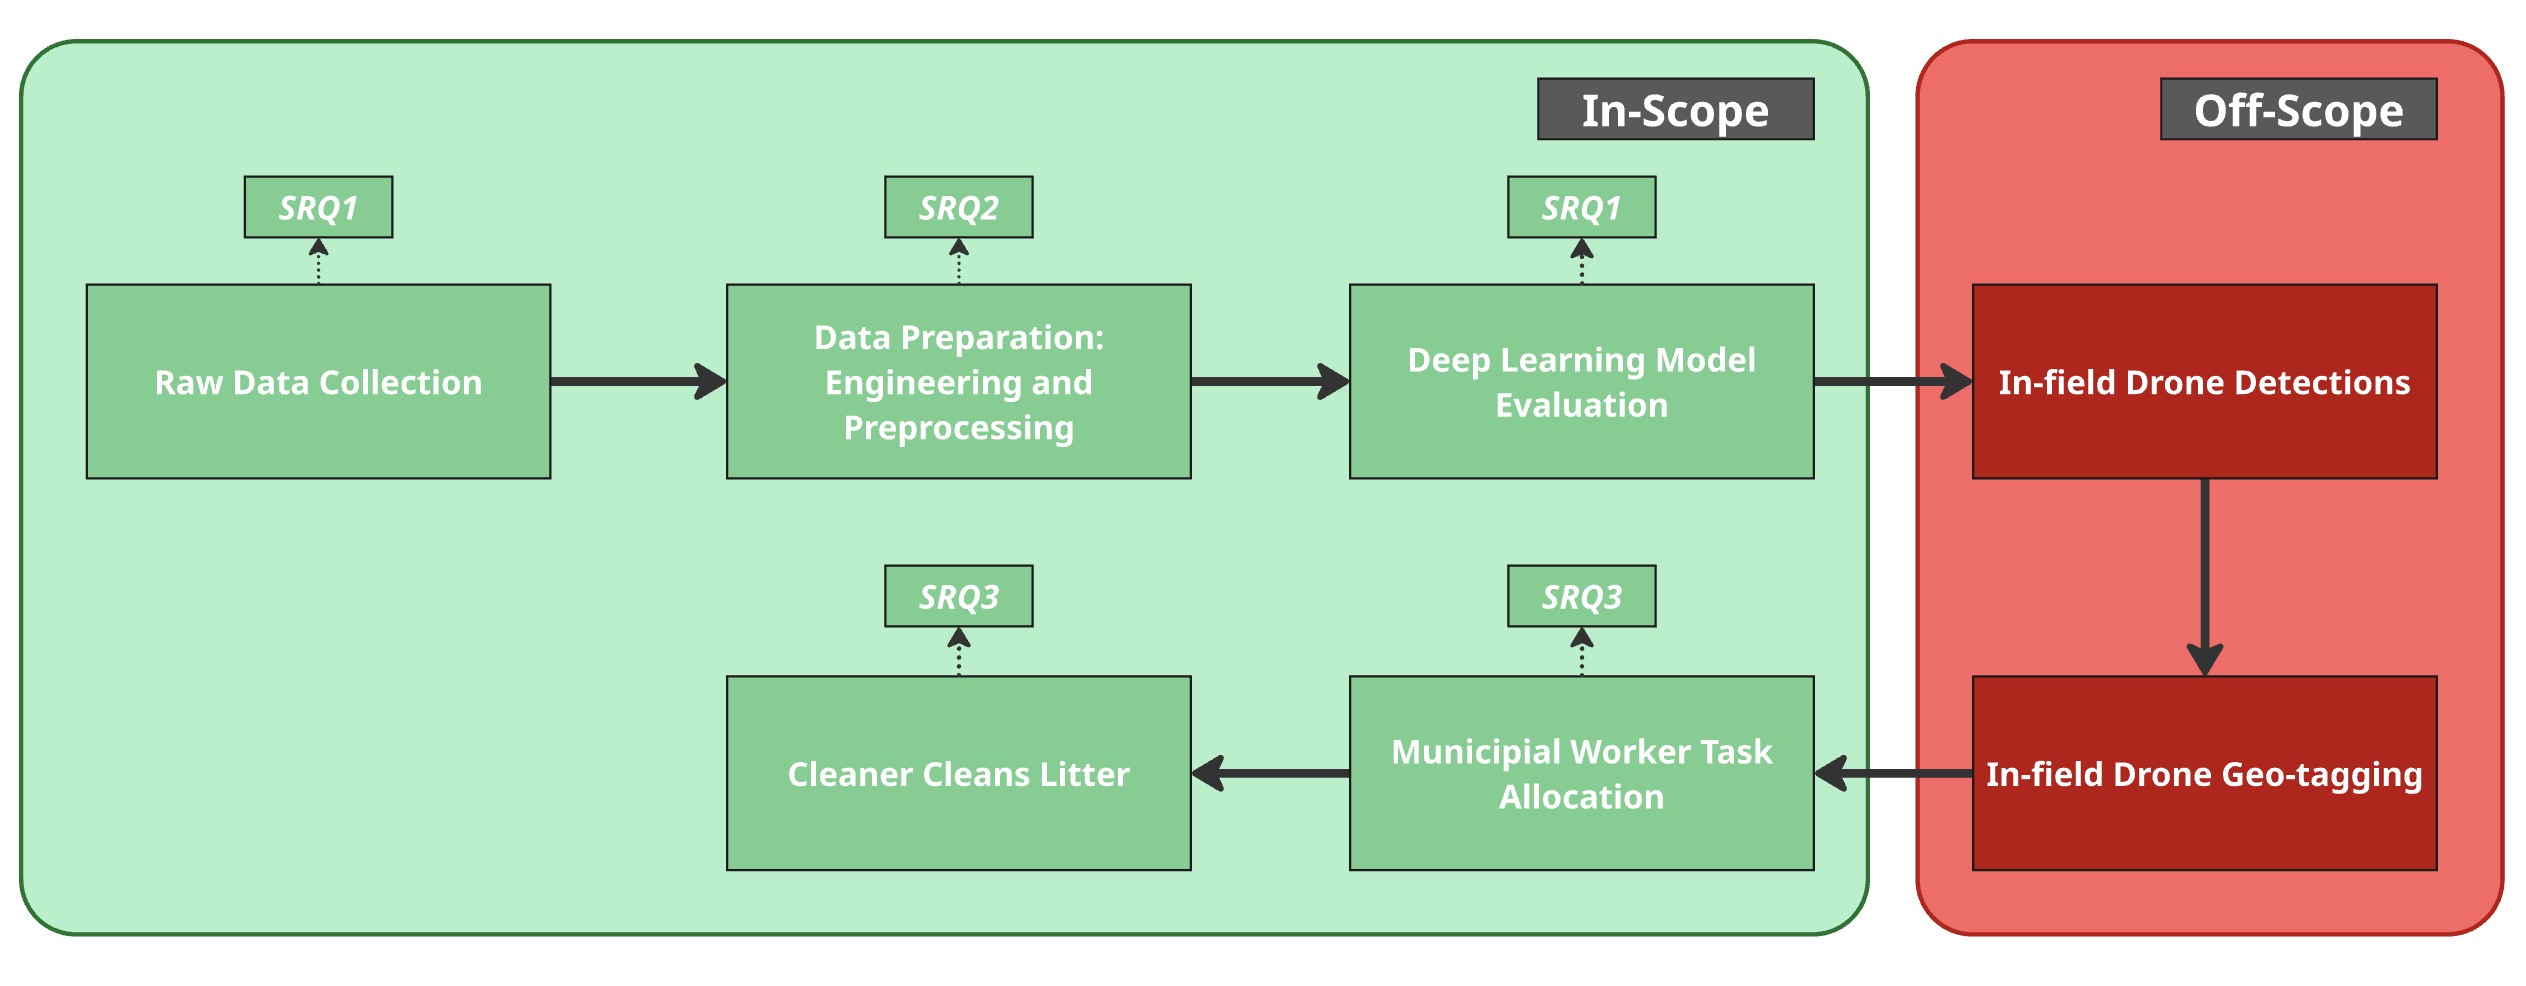
\includegraphics[width=0.8\linewidth]{system_scope.png}
    \caption{Project system scope and operational boundaries.}
    \label{fig:system_scope}
\end{figure}
While live field testing is ultimately necessary to achieve a fully automated UAV-litter solution, physical drone deployment was omitted from this study to ensure a rigorous, focused evaluation of the underlying software, dataset, and perceptual models. Further elaboration on this scoping decision is detailed in Section 9.1 (Project Management).
